\documentclass[a4paper,twoside]{IEEEtran}




% Löschen oder kommentieren Sie die folgenden beiden Zeilen aus,
% wenn Sie den Text in Englisch schreiben wollen.
\usepackage{german}
\usepackage[utf8]{inputenc}

\usepackage{graphicx}
\graphicspath{{figures/eps/}}
\usepackage{ dsfont }
\usepackage{ gensymb }
\usepackage{amsthm}
\usepackage{amsmath}

\newtheorem{boundedSpannerTheorem}{Theorem}[section]
\newtheorem{inwardPathProposition}{Proposition}




\newcommand{\seminarteilnehmer}{Tim Budweg}
\newcommand{\seminartitel}{Erklärung zum modified Yao-Step angewandt auf den Delaunay Graphen}

\begin{document}

\title{\seminartitel}
\author{\seminarteilnehmer}

\markboth{Seminar Rechnernetze, Wintersemester 2014/2015}%
{\seminarteilnehmer: \seminartitel}


\maketitle

\begin{abstract}
\space Diese Arbeit erläutert die Spannerbildung mithilfe der Delaunay-Triangulation und dem modified Yao-Step aus \cite{kanj}. Der \emph{stretch-factor} liegt bei 3.54 in Bezug zum Euklidischen Graphen und beschränkt den Ausgangsgrad der Knoten auf 14.
\end{abstract}

\begin{IEEEkeywords}
\space Spanner, ad-hoc Netze, Delaunay Graph, Modified Yao-Step
\end{IEEEkeywords}


\section{Einleitung}
Es gibt viele Anwendungsbereiche für drahtlose Sensornetze. 
Zum Beispiel können Waldbrände oder Tsunamis durch ein Sensornetz-Frühwarnsystem schneller erkannt werden. 
Sowohl in diesem Beispiel als auch in anderen Anwendungsgebieten ist es gewünscht, dass alle gesendeten Nachrichten ankommen.
Garantierte Nachrichtenauslieferung wird von mehreren Algorithmen bereits erreicht (z.B.: Face-Routing: siehe \cite{FaceRouting}).
Jedoch müssen dafür bestimmte Voraussetzungen an das Sensornetz erfüllt sein. 
Die wichtigste Voraussetzung ist die Planarität des Netzes, das heißt, dass keine \emph{Kantenschnitte} (siehe \ref{Kantenschnitt}) existieren dürfen. 
Diese Planarität zu erreichen ist ein wichtiges Ziel von \emph{Topologiekontrollen}.

Ein weiterer Punkt ist, dass diese Netze willkürlich groß werden können.
Deshalb führt ein \emph{zentralisierter} Algorithmus zu einer sehr langen Laufzeit mit hohem Energieverbrauch, weil die Menge der versendeten Nachrichten in Abhängigkeit zu der globalen Netzgröße steht.

Damit die Nachrichten nicht über beliebig lange Pfade geroutet werden müssen, wird eine Beschränkung der Pfadverlängerung gewünscht. 
Pfadverlängerungen entstehen, wenn (spezielle) kantenlöschende Algorithmen auf Graphen angewendet werden.
Der hier behandelte Algorithmus ist streng lokal, was die Anzahl der gesendeten Nachrichten minimiert.
Außerdem produziert dieser einen \emph{t-Spanner} des euklidischen Graphen.
%\textit{t-Spanner} geben den größtmöglichen Umweg an, der entsteht, wenn man einen (speziellen) kantenlöschenden Algorithmus auf einen Graphen anwendet.
Diese Thematik wird im Folgenden anhand des Artikel von \cite{kanj} erläutert.
Dort wurde ein streng lokaler Algorithmus aufbauend auf den \emph{Delaunay Graphen} angewandt.
Das Ergebnis ist ein Graph, welcher im Bezug zum euklidischen Graphen einen stretch-factor von $t=3.54 $ und zusätzlich eine Beschränkung des Ausgangsgrad eines Knoten von $k=14 $ hat.

\subsection{Kantenschnitte} \label{Kantenschnitt}
Ein Kantenschnitt ist ein Punkt, in dem sich zwei oder mehr Kanten desselben Graphen schneiden.


%Spanner?


%\subsection{Planarität}
%Ein Graph ist planar, wenn es keine zwei Kanten gibt, die sich schneiden.

\subsection{Graphen}
\subsubsection{Euklidischer Graph}
Ein euklidischer Graph ist ein spezieller Graph. 
Alle Knoten sind mit allen anderen Knoten verbunden (Clique) und die Kantengewichte entsprechen der euklidischen Distanz beider Eckpunkte. 
Ein Beispiel finden Sie in Abbildung \ref{fig:Graph}.
\begin{figure}[h!]
\centering
\includegraphics[width=0.99\linewidth]{Graph.eps}
\caption{Ein euklidischer Graph}
\label{fig:Graph}
\end{figure}
\subsubsection{Unit Disk Graph}
Der Unit Disk Graph ist ein euklidischer Graph ohne alle Kanten, die länger als ein konstantes $c \in \mathds{R} $ sind.
In Abbildung \ref{fig:UnitGraph} sehen Sie den euklidischen Graph aus Abbildung \ref{fig:Graph} als Unit Disk Graph mit $c = 1 $.
\begin{figure}[h!]
\centering
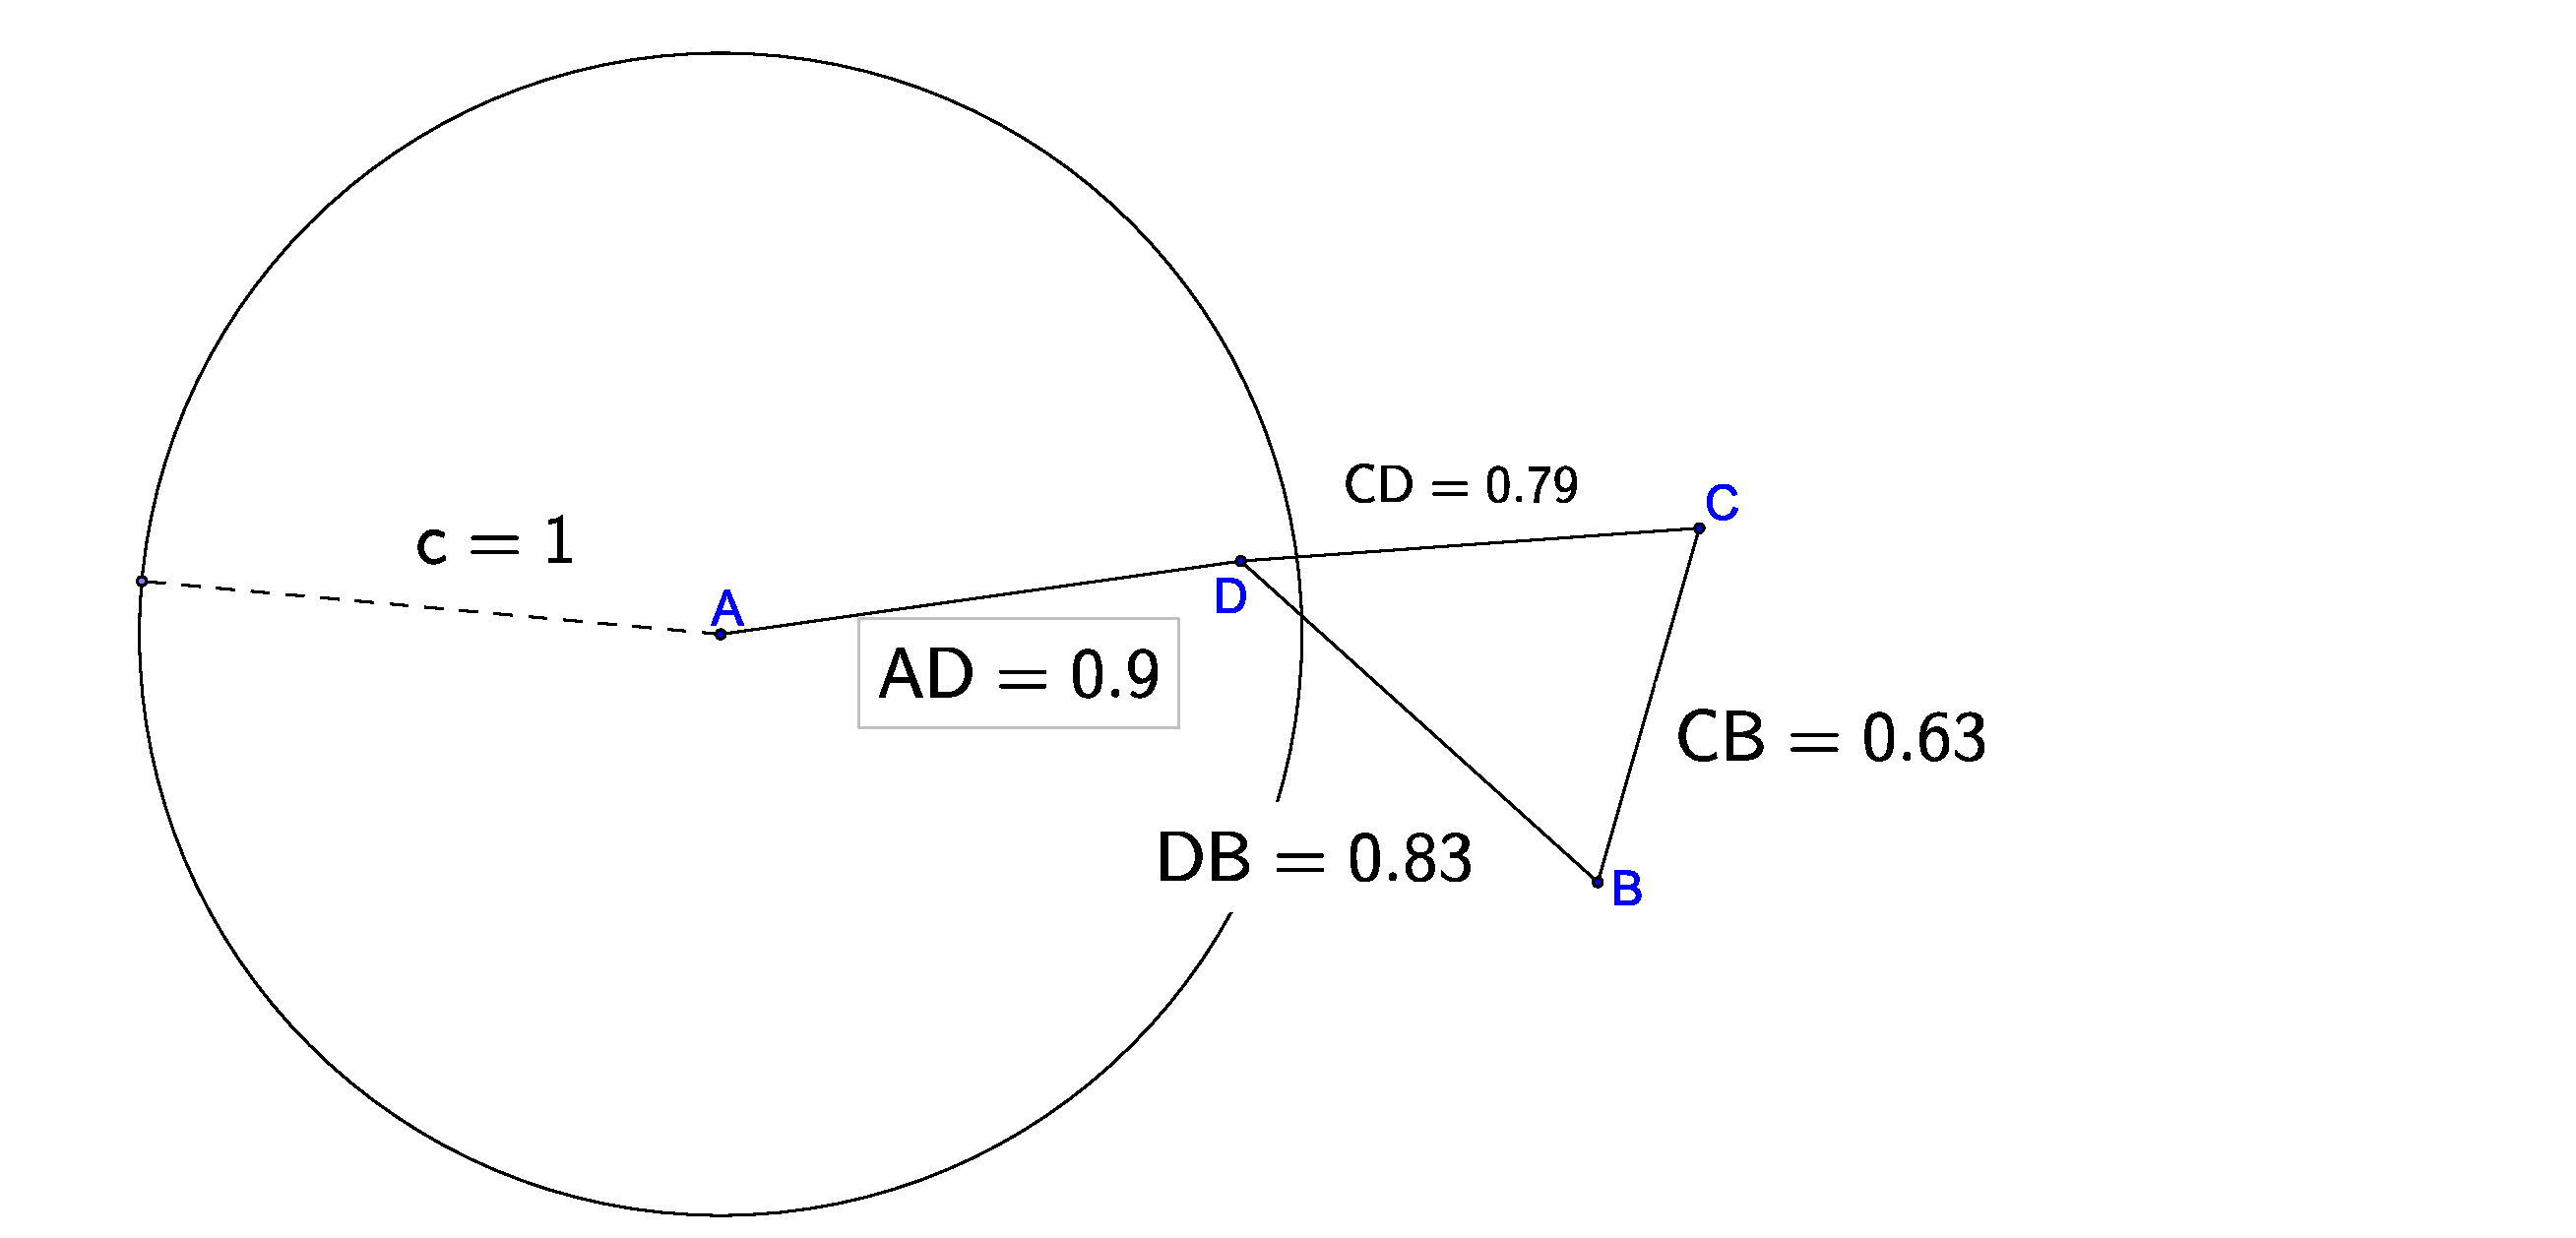
\includegraphics[width=0.99\linewidth]{UnitGraph.eps}
\caption{Der Unit-Disk-Graph zu Abbildung \ref{fig:Graph} mit $c = 1 $}
\label{fig:UnitGraph}
\end{figure}



\subsection{Spanner}
Gegeben ist ein Graph $G $, welcher ein Subgraph vom euklidischen Graphen $E $ ist.
$G $ enthält alle Knoten von $E $, aber nicht alle Kanten. 
Die Umwege, die durch das Löschen von Kanten entstehen, dürfen nur um einen konstanten Faktor ansteigen. 

\subsubsection{Euklidischer Spanner}
$H $ ist genau dann ein euklidischer Spanner von $G $, wenn die kürzesten Pfade zwischen allen Knoten maximal um einen konstanten Faktor $t $ vergrößert werden.
Die Notation $c_{G}(A, B) $ bedeutet: der kürzeste Pfad zwischen A und B im Graphen $G $.
Formal bedeutet das:
\begin{equation}
	c_H(A, B) \leq t \cdot c_G(A, B)
\end{equation}
{\footnotesize (Formel entnommen aus \cite{kanj} und angepasst)}

\subsection{Yao Step}
Gegeben ist ein Graph $G $. Für alle Knoten $A \in G $ wird folgender Algorithmus ausgeführt:
\begin{itemize}
\item Erzeuge k gleich große Kegel um $A $. $k \in \mathds{N} > 6 $
\item Bestimme die kürzeste Kante in jedem Kegel ausgehend von $C $.
\item Lösche alle Kanten, die nicht von beiden Endpunkten ausgewählt wurden.
\end{itemize}

\begin{figure}
\centering
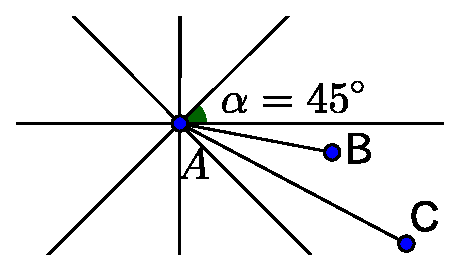
\includegraphics[width=0.99\linewidth]{Yao_Step2.eps}
\caption{Punkt C mit acht $45\degree $ großen Kegeln. Kürzeste Kante $AC $ wird ausgewählt}
\label{fig:YaoStep2}
\end{figure}


%Dadurch entsteht Graph $G' $. 

\subsection{Delaunay Triangulation}
Die Delaunay Triangulation erzeugt aus einem beliebigen zusammenhängenden Graphen einen geometrischen (= euklidischen) Spanner mit dem Streckungsfaktor $c_{del} \approx 2.42 $ und einem beliebig hohen Ausgangsgrad eines Knotens. 
Dazu werden alle Dreiecke betrachtet.
Wenn der Kreis durch alle Eckpunkte des Dreiecks keine weiteren Punkte des Graphen enthält, sind diese drei Kanten auch im Delaunay Graphen. 
Um Fallunterscheidungen zu vermeiden wird angenommen, dass keine vier Punkte auf einem Kreis liegen. 



\subsection{Synchronität}
Bei einem synchronen Algorithmus ist die Arbeitsweise der Knoten in Runden und diese in Phasen eingeteilt. 
Eine Runde sieht beispielsweise wie folgt aus:
\begin{itemize}
\item Zuerst erhalten alle Knoten ihre Nachrichten, falls es welche gibt.
\item Danach verarbeiten sie die Nachrichten und stellen ggf. weitere Berechnungen an.
\item Am Ende der Runde werden Nachrichten an andere Knoten verschickt.
\end{itemize}
Hier ist zu beachten, dass alle gesendeten Nachrichten zu Beginn der Folgerunde angekommen sind.

%Algorithmus, definieren, dass es sich hier um Algorithmen auf Graphen handelt?
\subsection{Lokale Algorithmen} \label{lokal}
Ein Algorithmus ist genau dann lokal, wenn jeder Knoten ausschließlich mit seiner \emph{k-Hop} Nachbarschaft kommuniziert. ($k \in \mathds{N}$)
Formal reicht dies aus, um einen Algorithmus lokal zu nennen.
Das Problem, dass der Algorithmus eine lange Laufzeit hat (siehe Einleitung), ist dadurch jedoch nicht gelöst.
Anhand des \emph{Maximal Independent Set (Fortan: MIS)} Algorithmus lässt sich ein Beispiel konstruieren, welches dieses Problem veranschaulicht.
%Es soll das \textit{Maximal Independent Set} (MIS) eines Graphen $G $ berechnet werden.
Betrachten Sie Abbildung \ref{fig:MIS}.

\begin{figure}[h!]
\centering
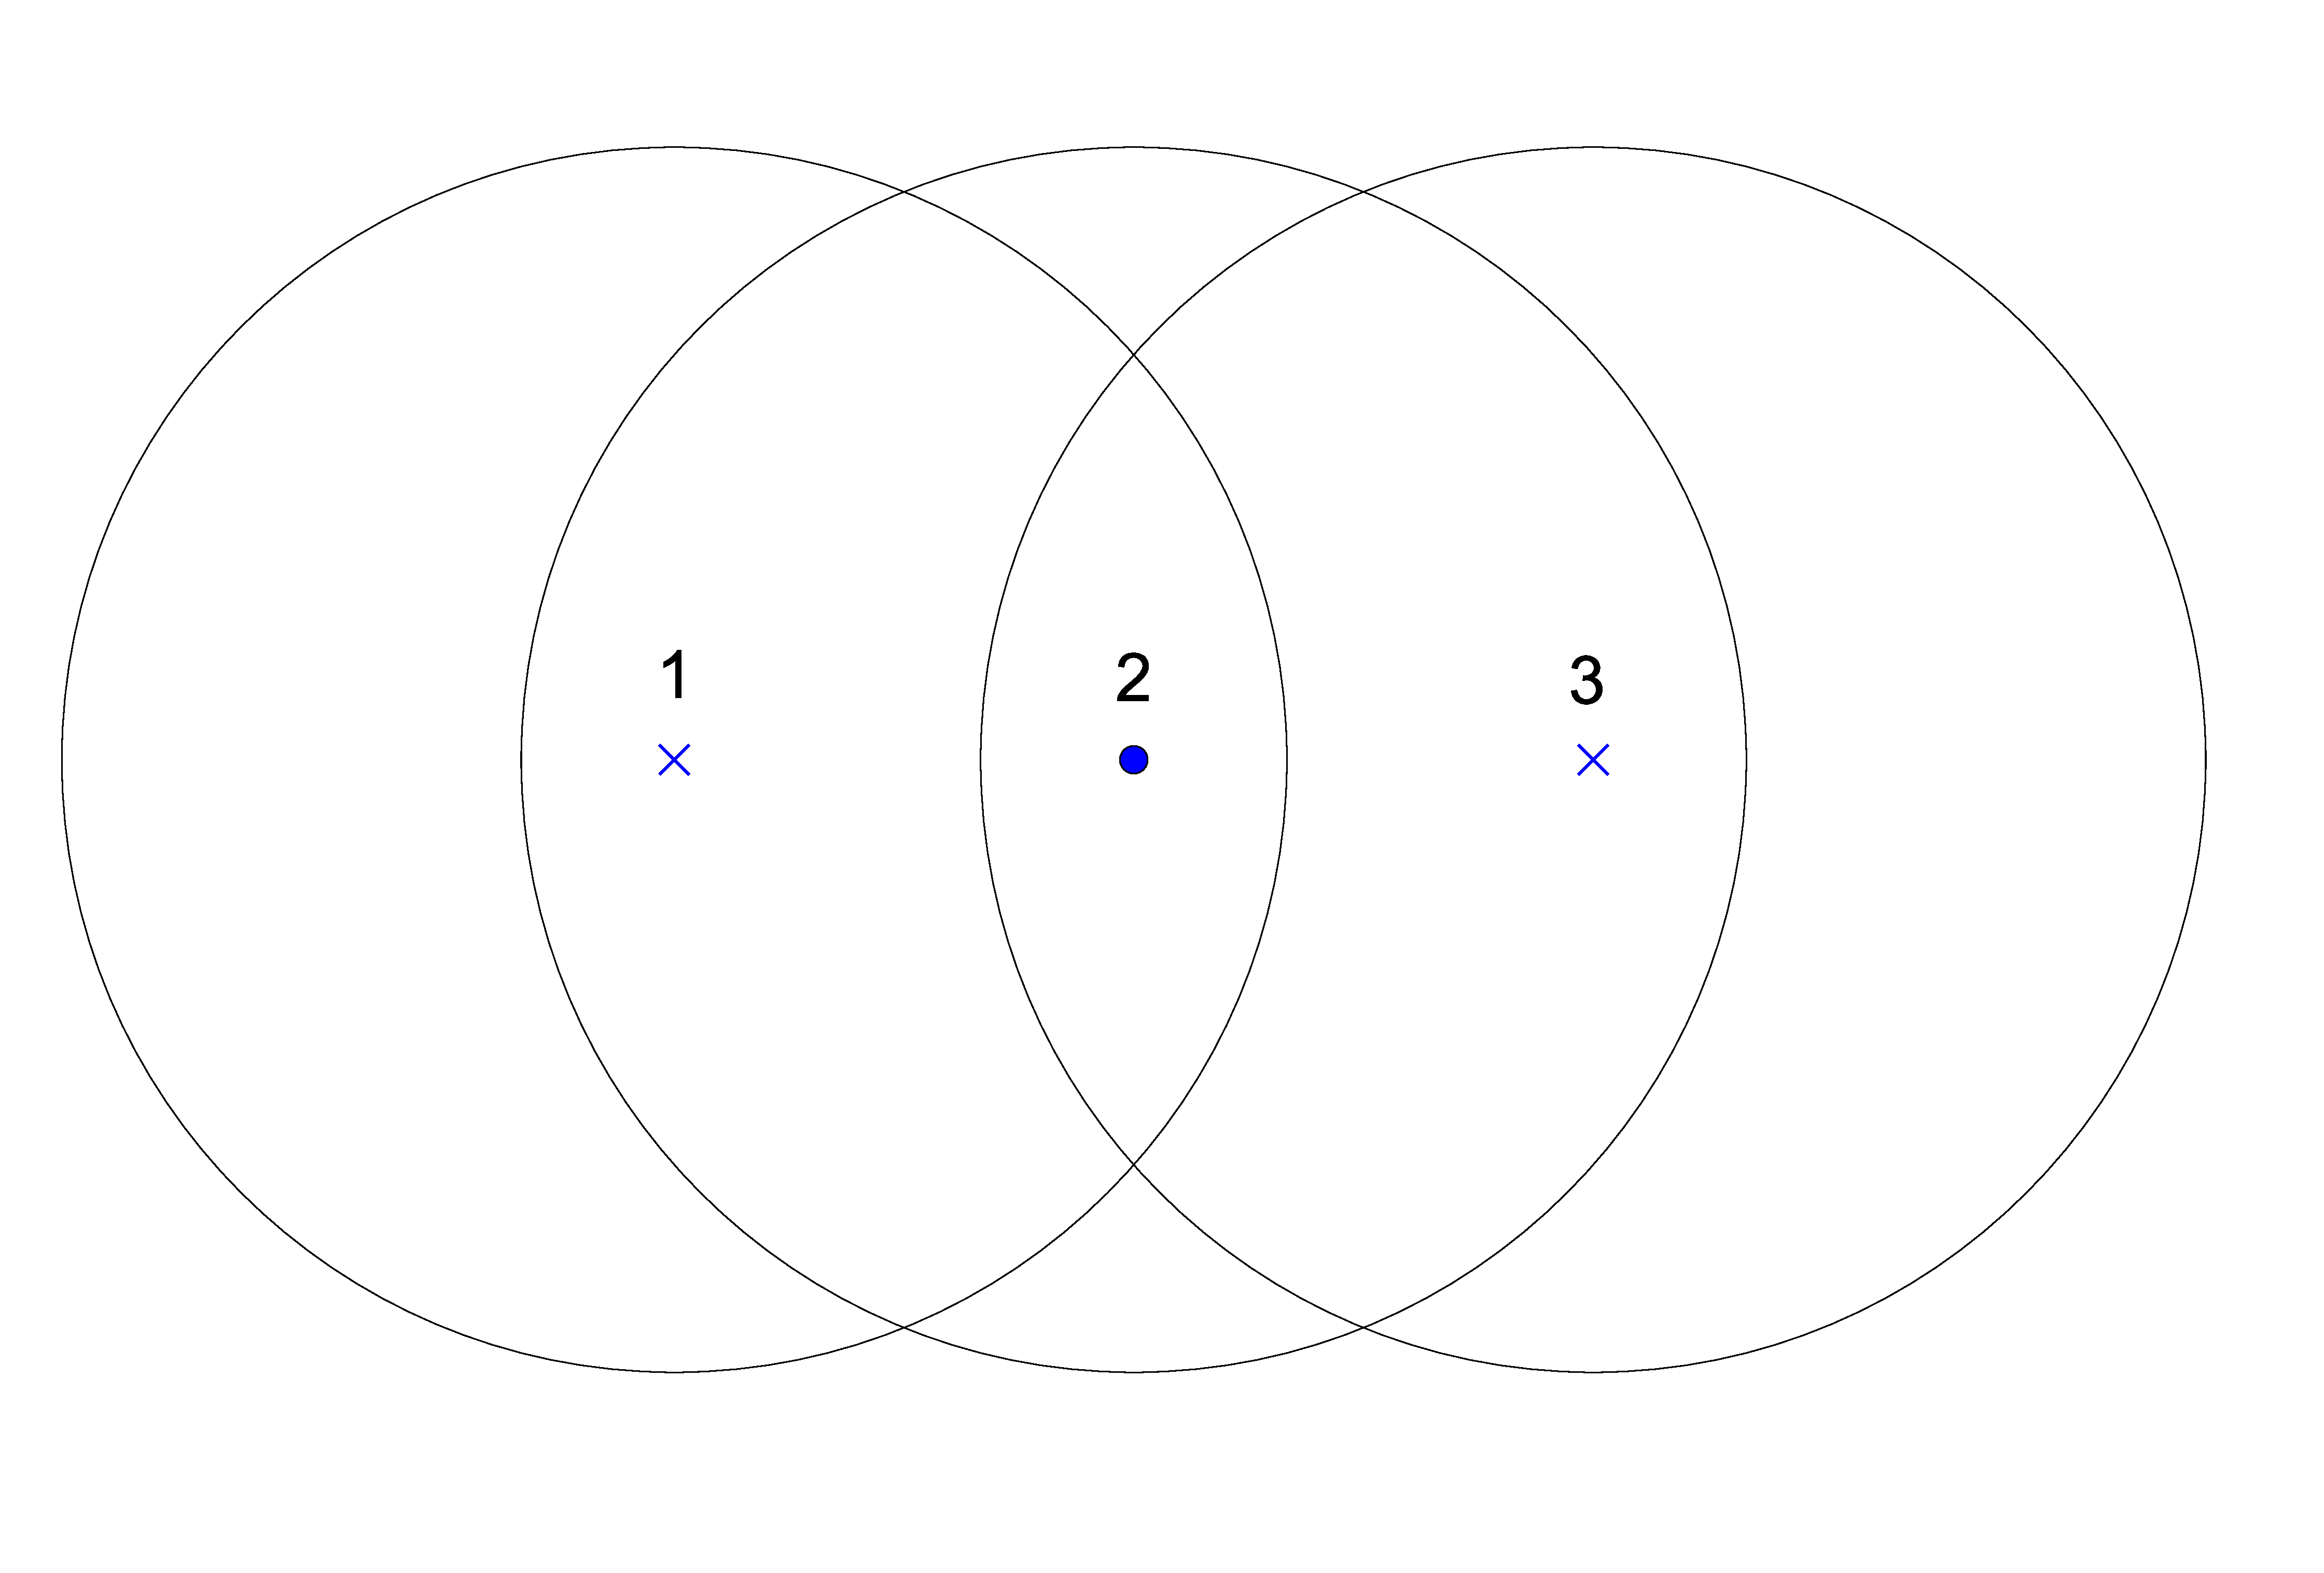
\includegraphics[width=0.99\linewidth]{MIS.eps}
\caption{$\times $ sind Knoten im Maximal Independent Set, $\bullet $ sind keine Knoten des MIS, Die Kreise um die Knoten sind die jeweiligen Sendebereiche.}
\label{fig:MIS}
\end{figure}


\begin{itemize}
\item \textbf{Runde 1}: Knoten 1 wird MIS-Knoten, da er von allen seinen Nachbarn, welche noch keine Rolle haben, derjenige mit der kleinsten ID ist. Knoten 2 und 3 warten, da es Knoten gibt, welche noch keine Rolle und eine kleinere ID haben.

\item \textbf{Runde 2}: Knoten 2 entscheidet, dass er kein MIS-Knoten ist, da er in seiner Nachbarschaft Knoten 1 kennt, der schon MIS-Knoten ist. Knoten 3 wartet.

\item \textbf{Runde 3}: Knoten 3 wird MIS-Knoten, da Knoten 2 kein MIS-Knoten ist und somit 3 die kleinste ID hat. 
\end{itemize}

Diese Schritte lassen sich durch den gesamten Graphen sukzessiv durchführen. 
Der Algorithmus hat demnach eine Laufzeit in der Größenordnung von 
\begin{equation*}
\theta (dia(G)) 
\end{equation*}
wobei $dia(G) $ für den Durchmesser (längster kürzester Pfad) des Graphen steht.

Die Definition des lokalen Algorithmus trifft hier zu, weil jeder Knoten nur mit seinen unmittelbaren Nachbarn, der 1-Hop-Nachbarschaft, kommuniziert.





\subsection{Strenge Lokalität}
Wie im Abschnitt \ref{lokal} beschrieben, sind lokale Algorithmen noch nicht ausreichend, um die benötigte Nachrichtenanzahl zu minimieren.
Strenge Lokalität ist gegeben, wenn ein \emph{synchroner} Algorithmus unabhängig von der Netzgröße in konstanter Zeit terminiert (siehe \cite{strictlyLocal}).



%\section{was erreicht diese Arbeit} %bearbeiten

\section{Geometrische Spanner}

Es gilt folgendes Theorem zu beweisen:

\begin{boundedSpannerTheorem}
Für jedes $k \geq 14 $ existiert ein Subgraph $G' $ vom Delaunay-Graph $G $, sodass $G' $ einen maximalen Ausgangsgrad von k und einen stretch-factor von $1+2\pi(k \cos{\frac{\pi}{k}})^{-1} $ hat.
\end{boundedSpannerTheorem}
Gegeben sind zwei Kanten $CA $ und $CB $ im Delaunay-Graph $G $ vom Euklidischen Graph $E $.
%$\bigcirc _{ABC}$ ist der Kreis durch die drei Punkte $A, B, C $
Ohne Beschränkung der Allgemeinheit sei $CA $ die kürzeste Kante.
Die Autoren von \cite{kanj} beweisen dieses Theorem mithilfe des \emph{outward} und des \emph{inward} Path. %, welche in 10 stehen...
Der outward Path kann gebildet werden, wenn kein Knoten von $G $ innerhalb von $\triangle {ABC} $ liegt.
Der inward Path verbindet die Knoten A und B, wenn Knoten innerhalb von $\triangle {ABC} $ liegen.

\subsection{Der outward Path}
Die Autoren von \cite{kanj} benutzen eine rekursive Definition um den Pfad von A nach B zu definieren.
Es gilt zu beweisen, dass dieser Pfad in jedem Fall existiert, weil anderenfalls der Graph nicht zwingend verbunden ist.
Dieser Fall darf nicht eintreten.
Außerdem muss nachgewiesen werden, dass die Länge dieses Pfades maximal
$1+2\pi(k \cos{\frac{\pi}{k}})^{-1} $ länger ist als der vorherige Pfad von A nach B.


\begin{itemize}
\item \textbf{Basisfall}: Die Rekursion endet, wenn $AB \in G $. (vgl. Abbildung \ref{fig:YaoStep2}: AB müssen verbunden sein, weil B der einzige Knoten in einem Kegel von A ist.)
\item \textbf{Rekursionsfall}: $AB \notin G $
\end{itemize}

Aufgrund der Delaunay-Eigenschaft, dass eine Kante nur dann nicht in $G $ enthalten ist, wenn im Kreis $\bigcirc {ABC} $ ein weiterer Punkt liegt, muss deshalb ein weiterer Punkt in  $\bigcirc {ABC} $ liegen.
Diesen Punkt nennen die Autoren von \cite{kanj} einen \emph{intermediate Point}.
Um den Pfad von A nach B zu erhalten, wird ein Pfad von A zum intermediate Point T und von diesem zu B erstellt und konkateniert (siehe Abbildung \ref{fig:intermediate}).
Dieser Rekursionsfall kann öfter eintreten, da es bezüglich A und T oder B und T einen weiteren intermediate Point $T' $ geben kann und dazwischen rekursiv fortführend bis der Basisfall eintritt.
Der Rekursionsfall bewahrt immer folgende Eigenschaften:
\begin{itemize}
\item $(O_1) $ und $(O_2) $ sind vollständig innerhalb von $(O) $ (vgl. Abbildung \ref{fig:outward_path_kreise})
\item $\alpha $ und $\beta $ sind beide kleiner als der Winkel $\angle {AOB} $ (vgl. Abbildung \ref{fig:outward_path_winkel}) 
\item Alle drei Winkel sind kleiner als $\frac{4\pi}{k} $
\end{itemize}

Abbildung \ref{fig:outward_path_fertig} zeigt ein Beispiel eines kompletten outward Path.

\begin{figure}[h!]
\centering
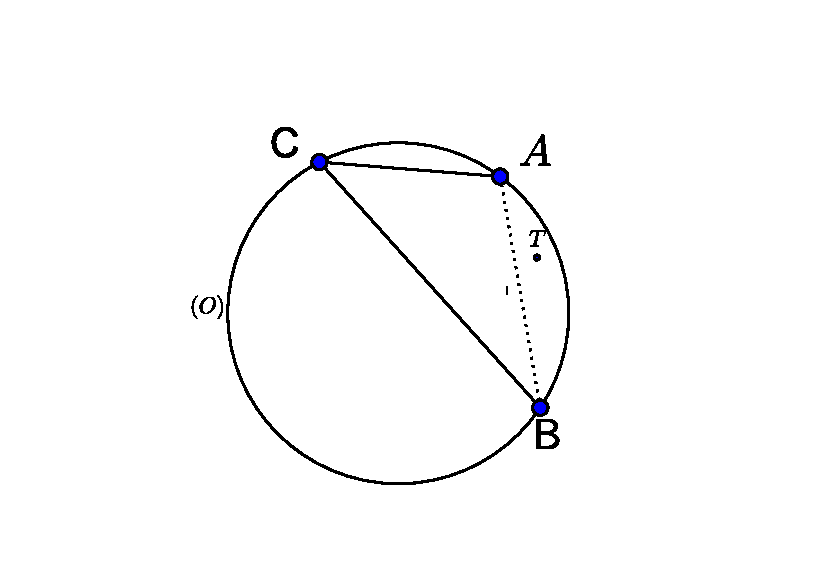
\includegraphics[width=1\linewidth]{outward_path1.eps}
\caption{T $\in G $ ist ein Knoten. Dieser Knoten wird intermediate Point mit Bezug zu $A $ und $B $ genannt.}
\label{fig:intermediate}
\end{figure}

\begin{figure}[h!]
\centering
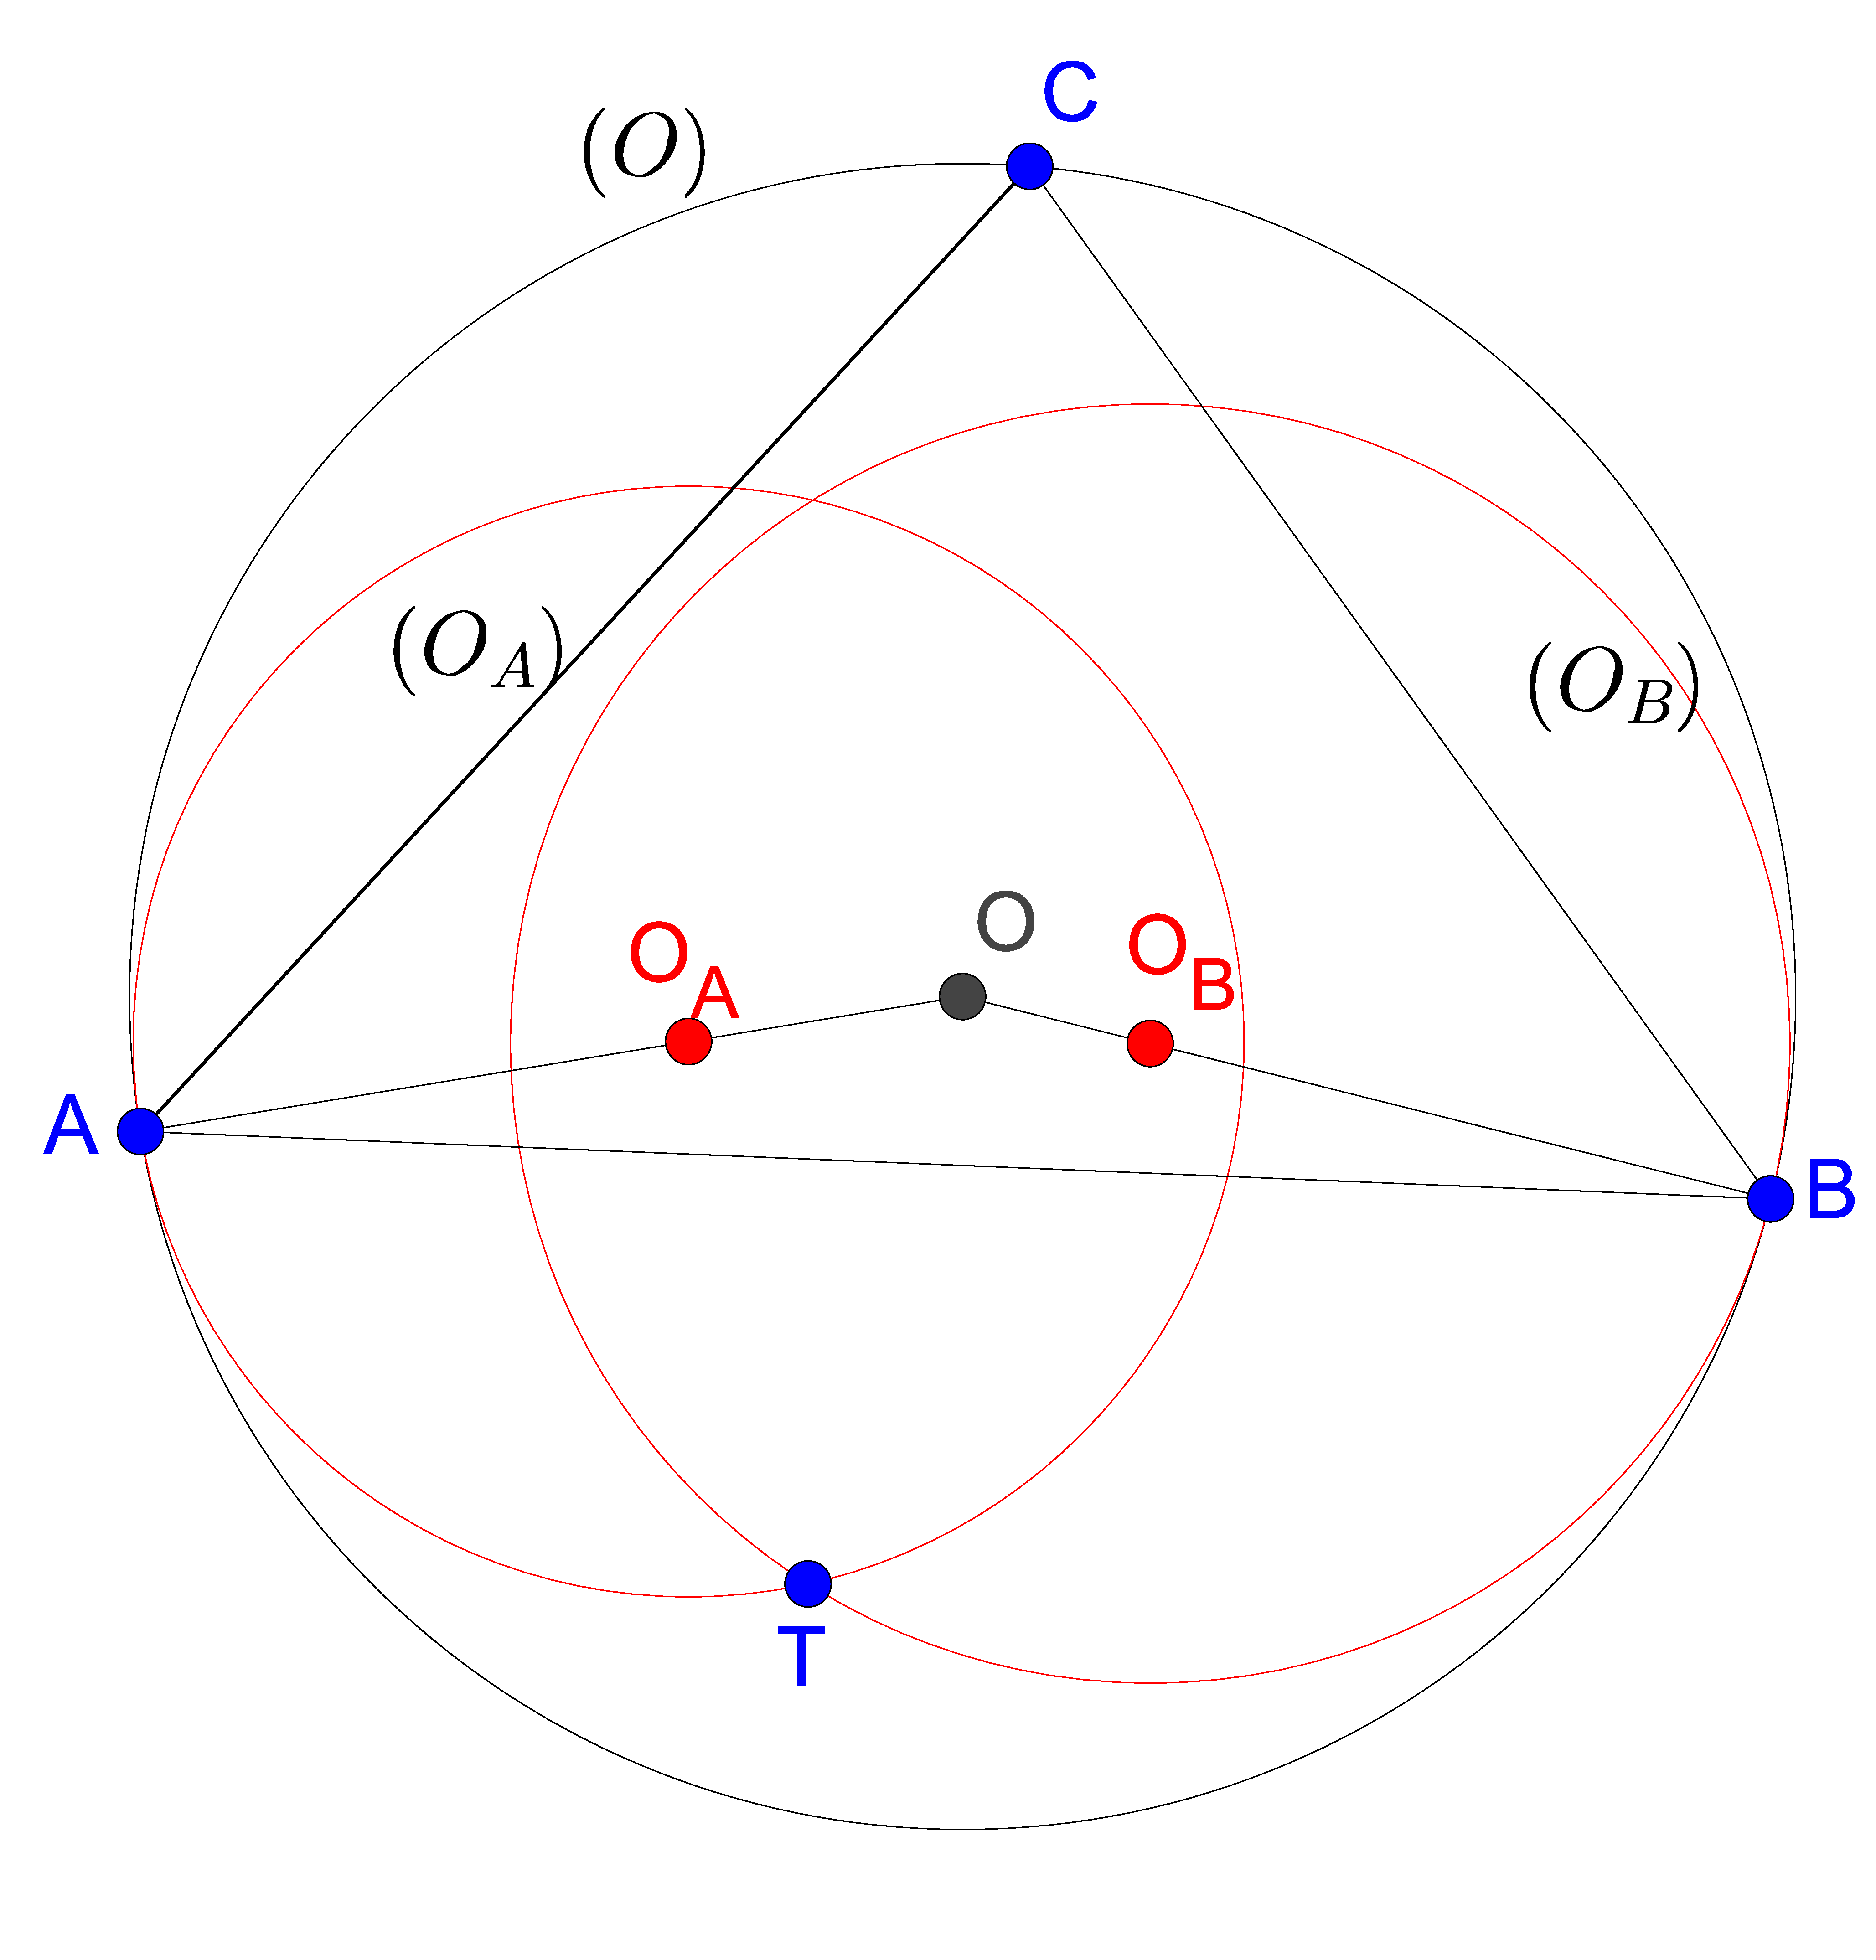
\includegraphics[width=0.8\linewidth]{outward_path_kreise.eps}
\caption{ $(O_1) $ und $(O_2) $ sind vollständig innerhalb von (O), $(O_1) $ ist der Kreis durch A und T mit Mittelpunkt auf dem Segment $AO $, $(O_2) $ verläuft durch B und T und der Mittelpunkt liegt auf dem Segment $BO $} 
\label{fig:outward_path_kreise}
\end{figure}

\begin{figure}[h!]
\centering
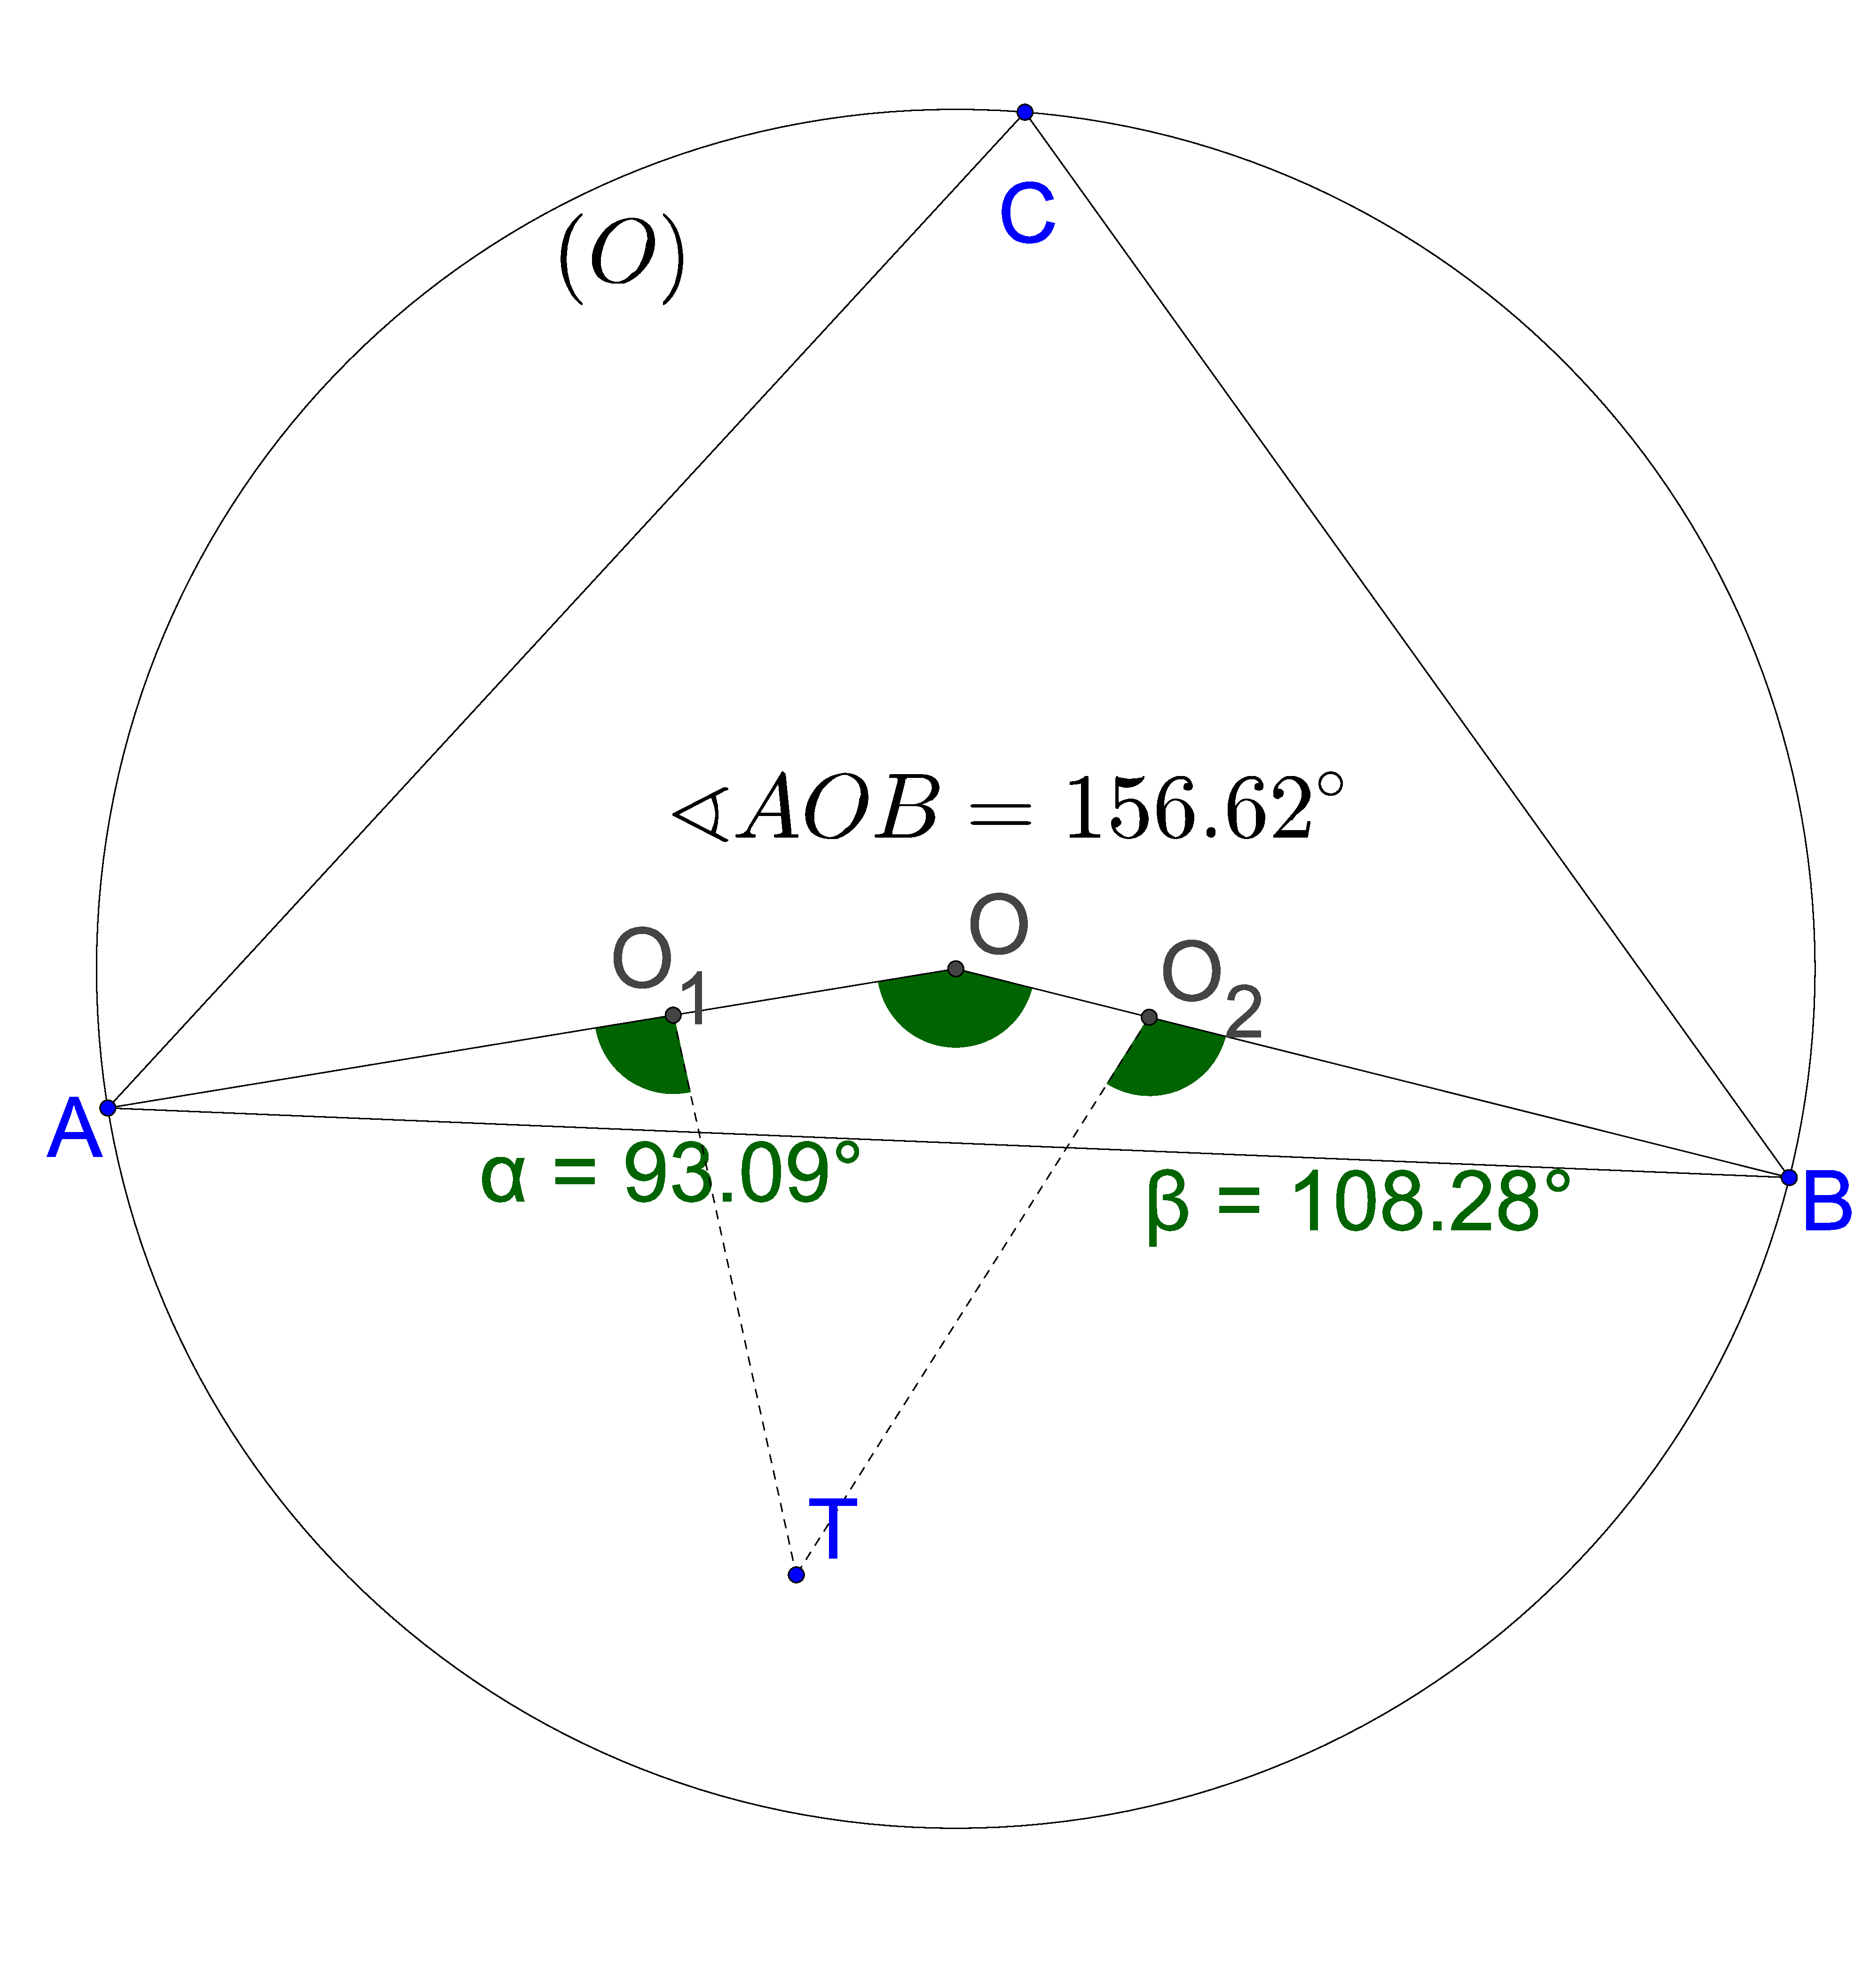
\includegraphics[width=0.8\linewidth]{outward_path_winkel.eps}
\caption{ $\alpha $ und $\beta $ sind beide kleiner als $ AOB $, gleiche Konstruktion wie in Abbildung \ref{fig:outward_path_kreise}, A und B liegen im selben Kegel ausgehend von C.}
\label{fig:outward_path_winkel}
\end{figure}

\begin{figure}[h!]
\centering
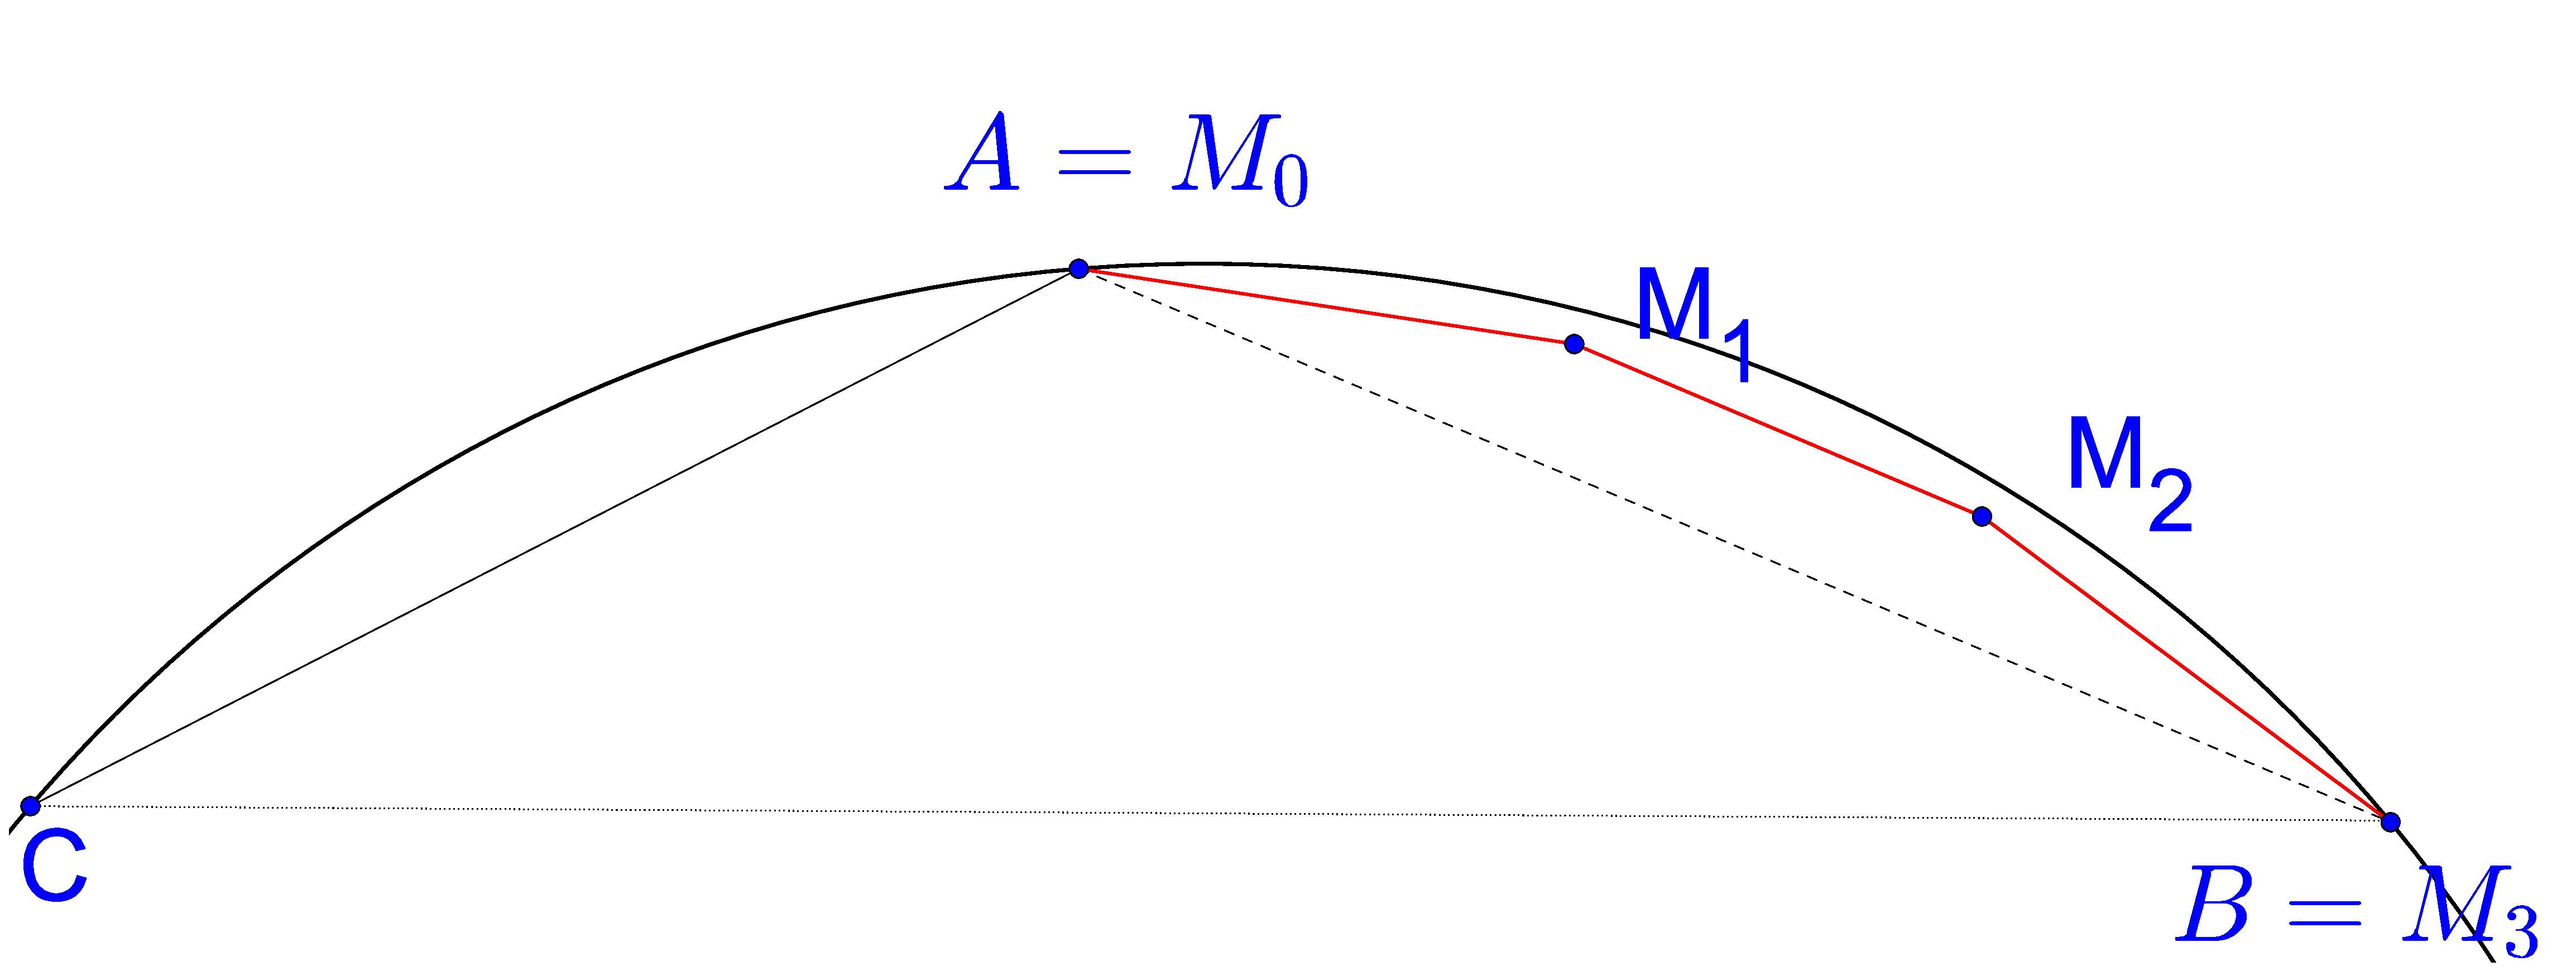
\includegraphics[width=1\linewidth]{outward_path_fertig.eps}
\caption{Zwischen $A $ und $B $ ist ein fertiger Outward Path mit den Intermediate Points $M_1 $ und $M_2 $}
\label{fig:outward_path_fertig}
\end{figure}

\subsubsection{Beweis}
Es wird behauptet, dass von A nach B ein Pfad $p $ existiert, sodass:
\begin{equation}
|CA| + |p| \leq (1+2\pi(\cos{\frac{\pi}{k}})^{-1})|CB|
\end{equation}
In Worten: Die Länge des Pfades $p $ plus den Wert $|CA| $ darf nicht größer sein als eine Konstante ($t \approx 1.45 $ für $k=14 $) multipliziert mit der Länge der Kante $CB $.
%Diese Konstante ist die maximale Länge des Teilstücks des Kreises $\bigcirc{ABC} $ von A nach B.

%\begin{figure}[h!]
%\centering
%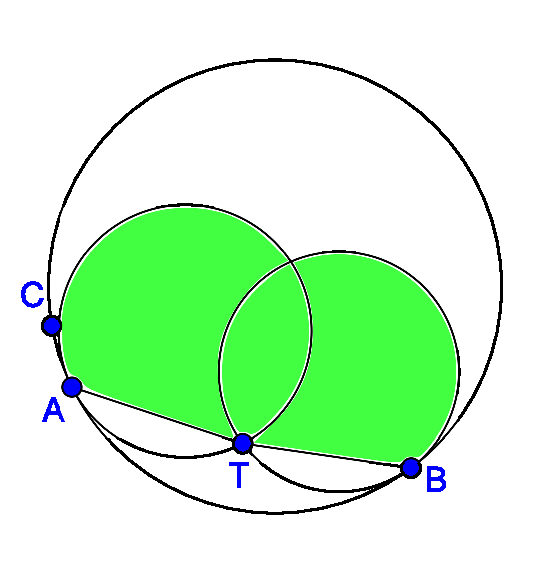
\includegraphics[width=0.8\linewidth]{outward_path_empty.eps}
%\caption{Die grünen Bereiche enthalten keine Punkte des Graphen.}
%\label{fig:outward_path_empty}
%\end{figure}






\subsection{Der inward Path}
Die Menge S besteht aus allen Punkten innerhalb von $\triangle {ABC} $, Punkt A und Punkt B.
In Abbildung \ref{fig:inward_path_prop} ist ein Beispiel eines Inward Path.
$CH(S) $ sind alle Punkte der Konvexen Hülle von S. %erklärung der konvexen hülle
Folgende drei Voraussetzungen gelten:
\begin{inwardPathProposition}
\begin{itemize} %TODO: funktioniert nicht.. erste zeile frei
	\item $CN_i \in G$
	\item $|CN_i| \leq |CN_{i+1}| $
	\item $\angle{N_{i-1}N_iN_{i+1}} \geq \pi $ (Winkel Richtung C)
\end{itemize} 
\end{inwardPathProposition}

Abbildung \ref{fig:inward_path_prop} zeigt, dass alle Winkel $\angle{N_{i-1}N_iN_{i+1}} $ größer als $\pi $ sind.
Außerdem ist jede Kante $CN_i $ kürzer als $CN_{i+1}$. 
Da CA ($= CN_0 $) die kürzeste Kante in diesem Kegel ist, muss $CN_1 $ länger sein. 
Für $CN_1 $ gilt dieselbe Bedingung. 
Folglich muss $CN_2 $ länger sein, etc.
Hinzu kommt die Voraussetzung $\angle{N_iCN_{i+1}} \leq \angle{BCA} $.
Dies sind genau die Bedingungen, welche im Voraus bewiesen wurden, um einen outward Path zu konstruieren. 
Zwischen jedem Paar $N_iN_{i+1} $ gibt es einen outward Path, der dieses Paar verbindet.
Diese gesamte Konstruktion, der Pfad von A nach B, wird inward Path genannt.

\begin{figure}[h!]
\centering
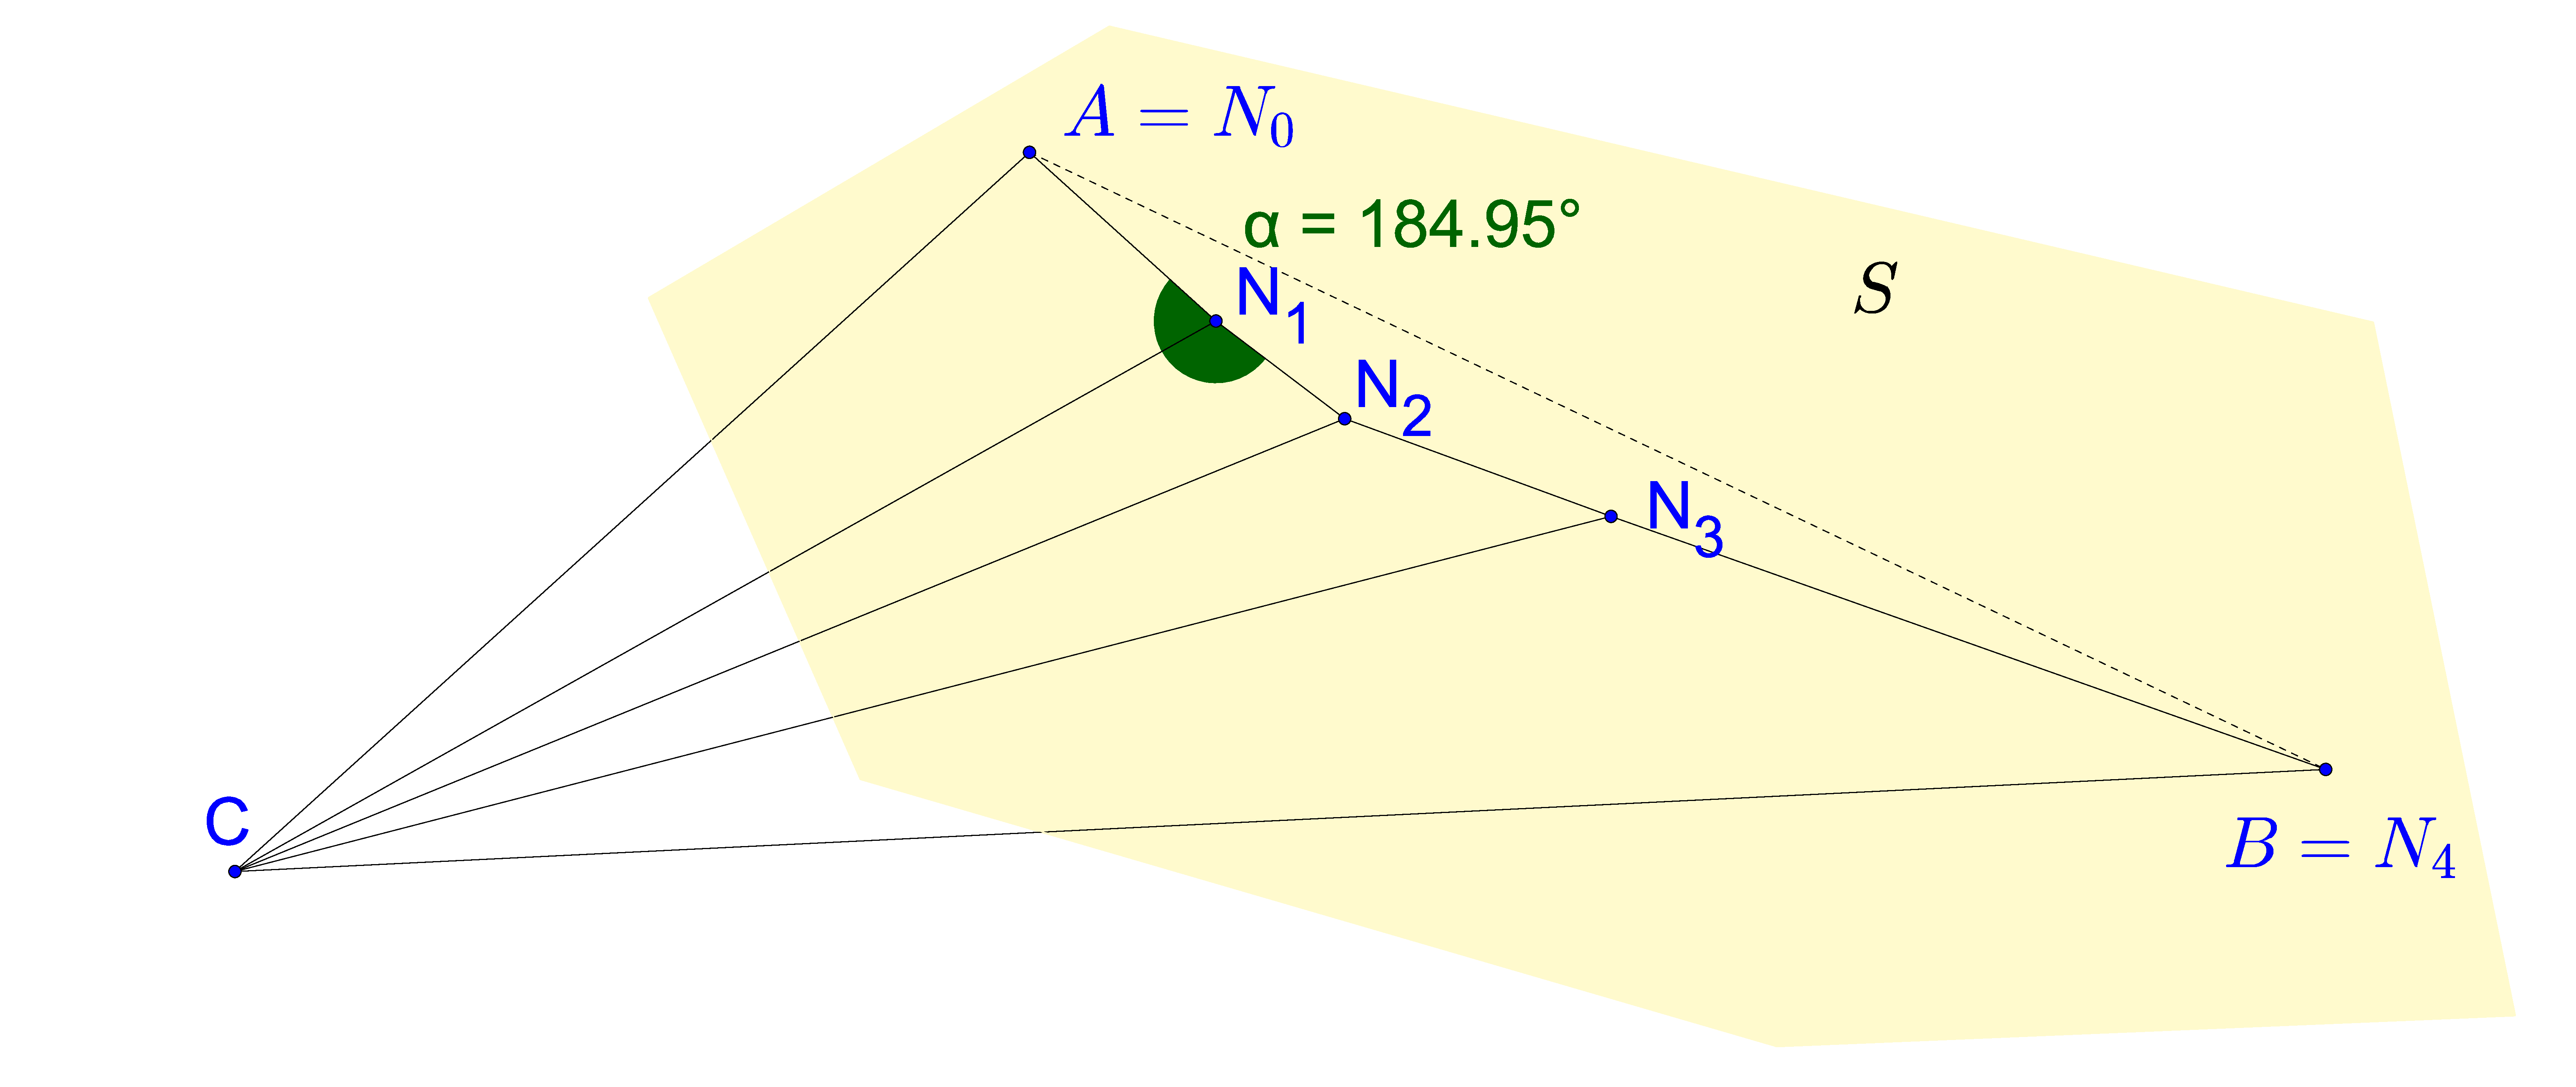
\includegraphics[width=1\linewidth]{inward_path_prop.eps}
\caption{Voraussetzungen für den inward Path und Beispiel eines inward Path $N_0N_1N_2N_3N_4 $}
\label{fig:inward_path_prop}
\end{figure}


\subsubsection{Beweis}



%$CH(S) $ ist die konvexe Hülle von S.
%$CH(S) $ enthält somit alle 
%\begin{figure}[h!]
%\centering
%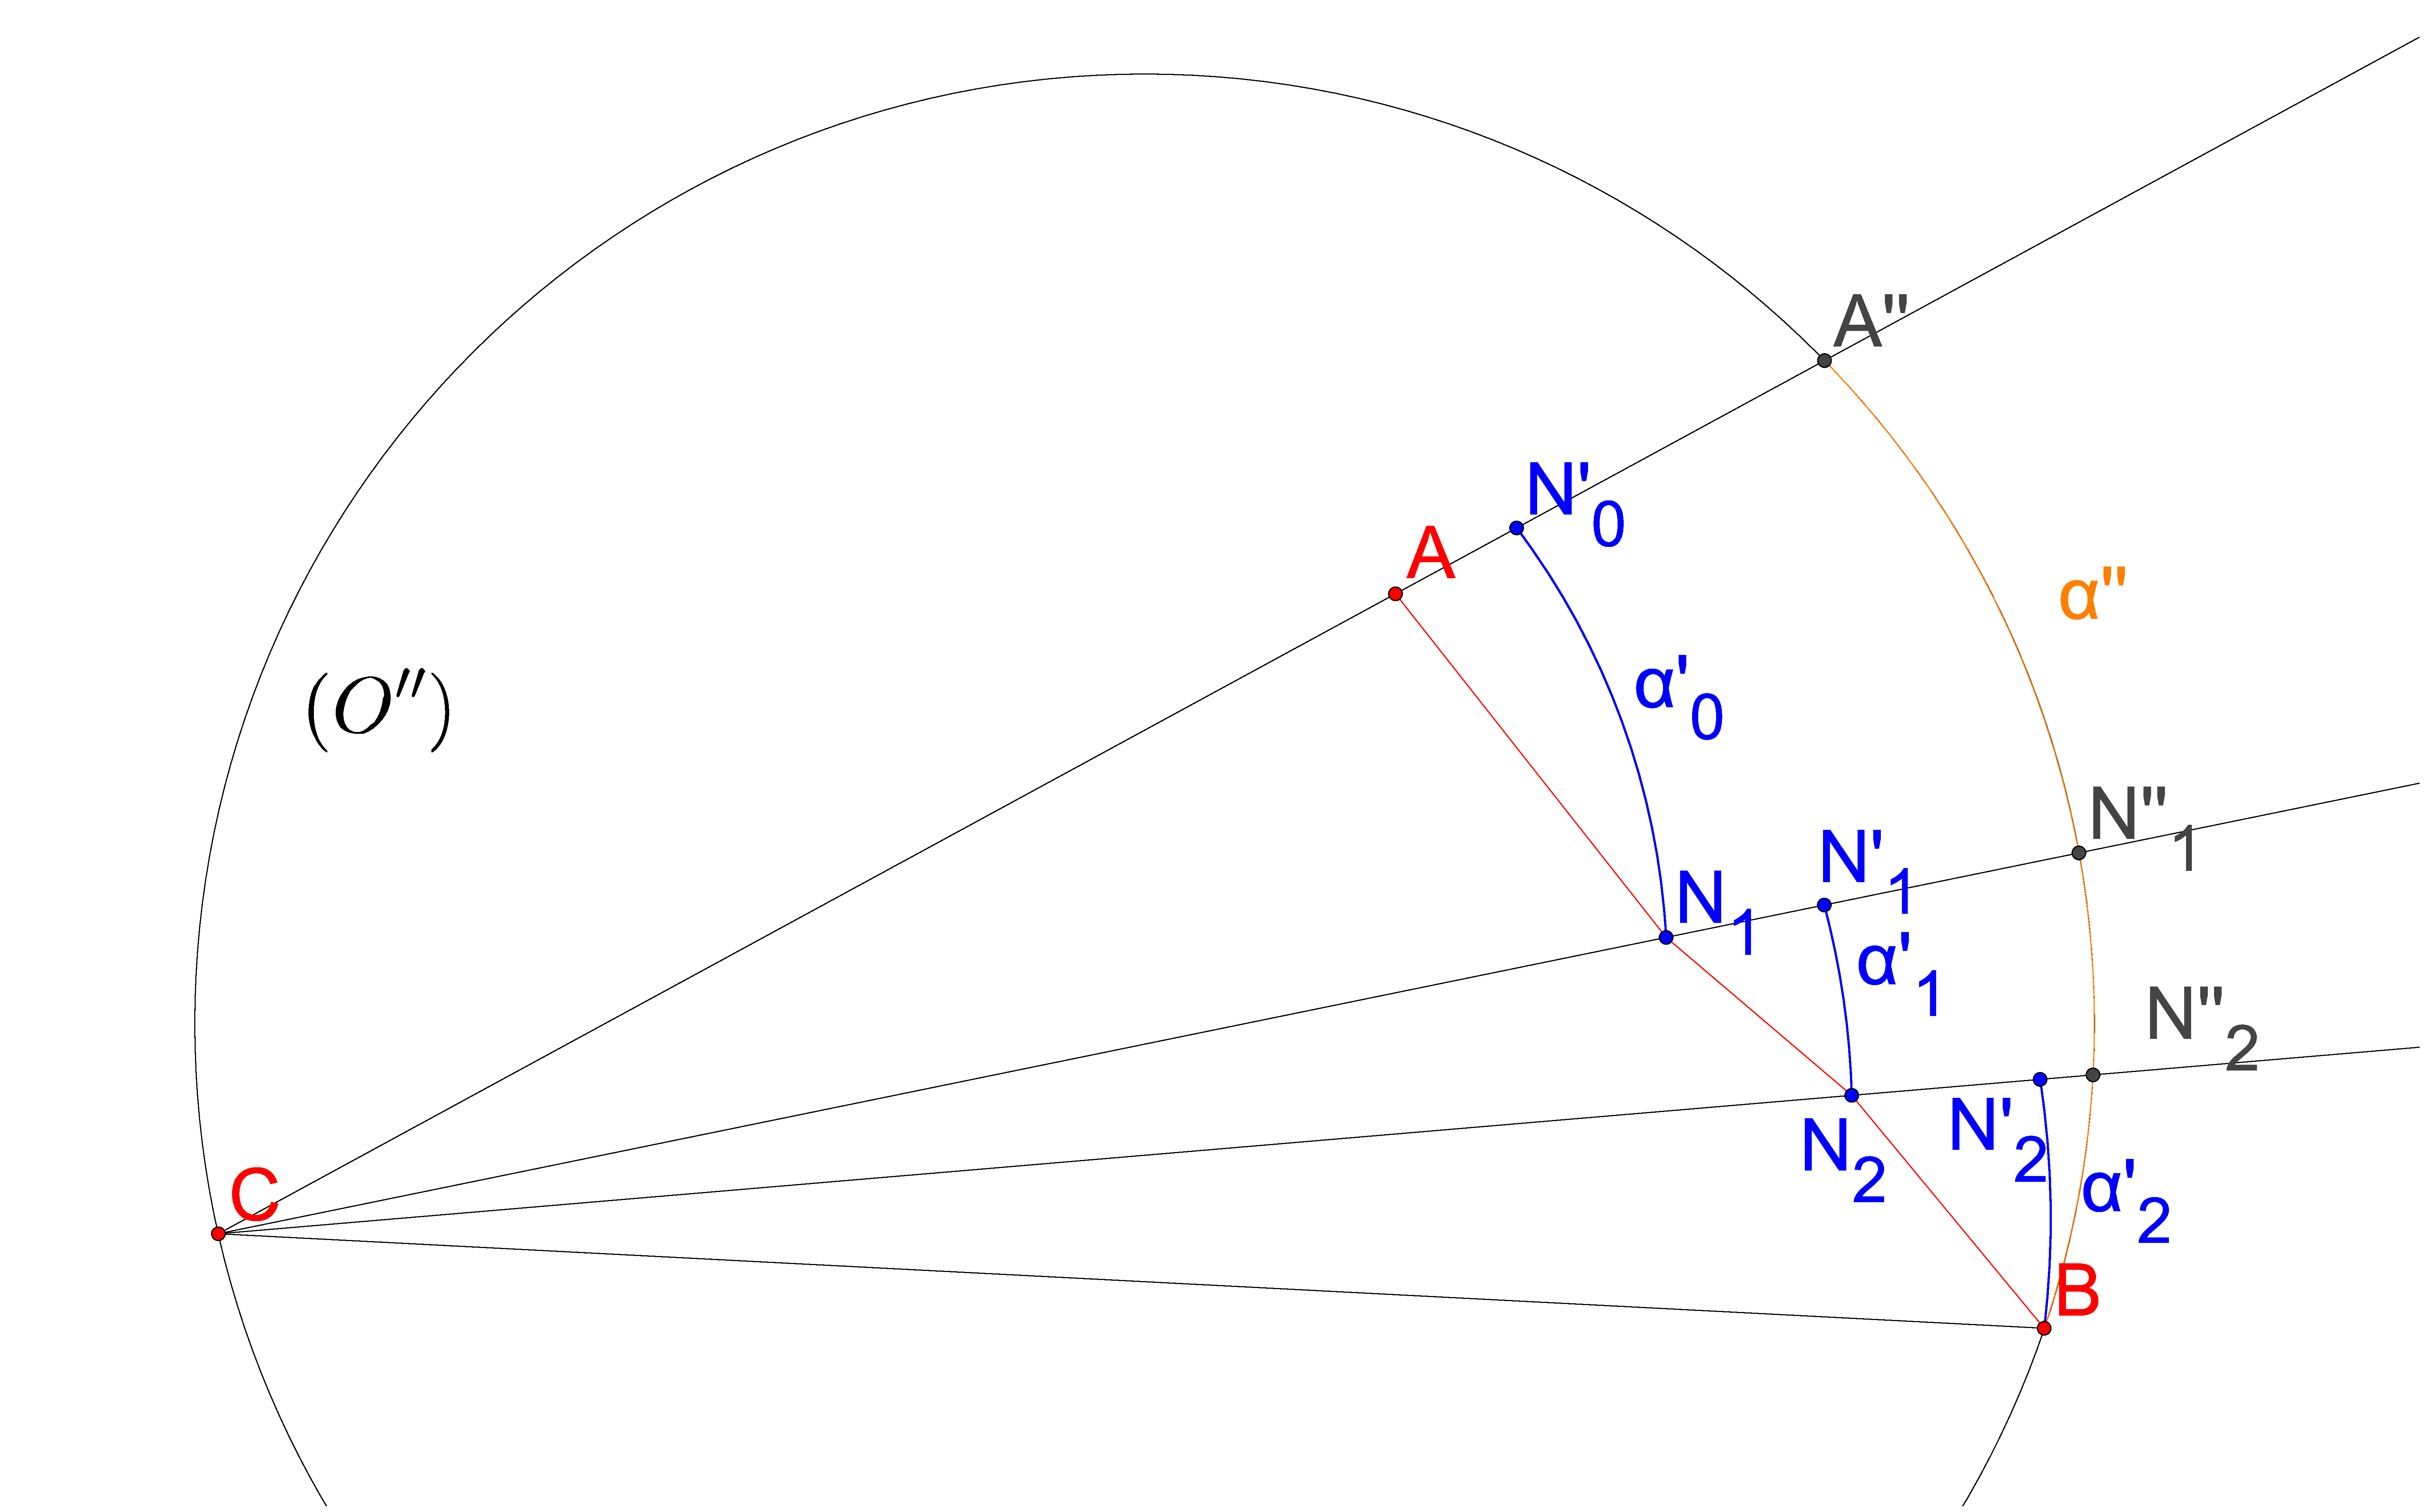
\includegraphics[width=1\linewidth]{inward_path1.eps}
%\caption{$AN_1N_2B $ ist der inward Path von A nach B}
%\label{fig:inward_path1}
%\end{figure}

%\section{Fazit}



\bibliographystyle{IEEEtran}
\bibliography{biblio}


\end{document}
